\chapter{Projekt systemu i opis narzędzi}
\label{DesignSystemChapter}
W poniższym rozdziale zostaną zaprezentowane kluczowe decyzje projektowe oraz założenia, jakie zostały przyjęte w toku prac nad implementacją systemu. Oprócz tego zostanie również przedstawiony opis narzędzi, które zostały wykorzystane do stworzenia aplikacji.

\section{Projekt systemu}
W fazie projektowania należy zdefiniować główne założenia projektowe oraz odpowiednio zaprojektować architekturę systemu. Podsumowując wyniki uzyskane w tej fazie, zdecydowałem się rozpatrzeć trzy najważniejsze zagadnienia:
\begin{enumerate*}
\item Definicja \textbf{rozwiązywanego problemu},
\item Lista \textbf{celów i założeń systemu},
\item \textbf{Architektura systemu}, rozpatrywana na najwyższym poziomie abstrakcji.
\end{enumerate*}

\subsection{Definicja rozwiązywanego problemu}
Zaprojektowany system powinien rozwiązywać problem treningu agentów sterujących samochodem wymodelowanym w środowisku symulacji. Samochód powinien pokonywać wyznaczony tor wyścigowy w możliwie najkrótszym czasie. Agenci odbierają informacje o swoim aktualnym położeniu dzięki obrazowi z jednej lub kilku kamer doczepionych do samochodu. W odpowiedzi na te informacje, do środowiska symulacji wysyłane są żądania podjęcia określonych zachowań, np. zmiany poziomu wciśnięcia pedału hamulca. Ponadto, środowisko symulacji na bieżąco przyznaje agentom nagrody i kary w zależności od tego, jak dobrze (lub źle) agent radzi sobie z postawionym zadaniem. Odpowiedni system kar i nagród jest kluczowy dla osiągnięcia zadowalających wyników treningu.

Agentami są konwolucyjne sieci neuronowe, a ich parametry są dostrajane przy użyciu metody uczenia maszynowego zwanej \textbf{uczeniem ze wzmocnieniem} (z ang. \textit{reinforcement learning}) \cite{deepRL:guide}.

\subsection{Cele i założenia}
\begin{enumerate*}
\item Stworzony system powinien być możliwie prosty w obsłudze.
\item Wytrenowane modele powinny być zapisywane do pliku o ustalonym formacie. Format pliku musi być rozpoznawany i obsługiwany przez aplikację.
\item Dane konfiguracyjne powinny być dostarczane z zewnętrznego pliku o ustalonym formacie.
\item System powinien zapisywać przebieg treningu sieci neuronowych w postaci plików dziennika. Pliki te powinny zawierać informacje ułatwiające późniejszą analizę treningu.
\item System powinien posiadać możliwość podglądu ,,na żywo'' postępów treningu sieci podczas jego trwania.
\end{enumerate*}

\subsection{Architektura systemu}
System składa się z dwóch zasadniczych modułów: Środowiska Uczenia oraz narzędzia \texttt{mlagents\_learn}. Moduły komunikują się ze sobą za pośrednictwem mechanizmu komunikacji dostarczanego przez zestaw Unity ML-Agents. Więcej informacji na temat każdego z modułów można uzyskać w rozdziale \ref{ImplementationChapter}-tym, poświęconym opisowi implementacji systemu.

\begin{figure}[h]
\begin{center}
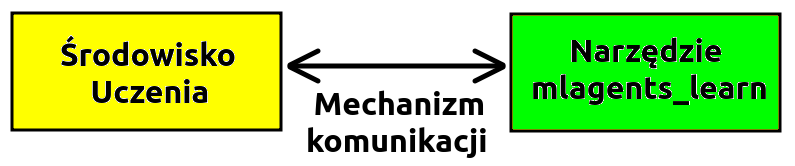
\includegraphics[width=15cm]{resources/figures/system_architecture.png}
\caption{Wizualizacja architektury systemu}
\label{SystemArchitecture}
\end{center}
\end{figure}

\section{Opis narzędzi}
W tej sekcji zamieszczam opis narzędzi wykorzystanych do implementacji systemu.
\subsection{Unity}
Multiplatformowy silnik gier 2D i 3D \cite{unity:opis}, napisany w językach C/C++.
Skrypty silnika należy pisać w języku C\#.
Gry tworzone na silniku Unity mogą być uruchamiane na bardzo wielu platformach sprzętowych i systemowych \cite{unity:buildTargets}:
\begin{enumerate*}
\item Komputery osobiste (PC):
\begin{itemize*}
\item Windows,
\item Linux,
\item Mac OS X;
\end{itemize*}
\item Urządzenia mobilne (smartfony):
\begin{itemize*}
\item Android,
\item iOS;
\end{itemize*}
\item Konsole do gier:
\begin{itemize*}
\item PlayStation 4,
\item PlayStation 5,
\item Xbox One,
\item Nintendo Switch;
\end{itemize*}
\item i wiele innych.
\end{enumerate*}

Unity posiada bardzo atrakcyjne warunki licencyjne - niemal wszystkie funkcje silnika są dostępne za darmo dla twórców nieprzekraczających 100 tysięcy dolarów rocznego dochodu.

W Unity powstało wiele popularnych gier, takich jak:
\begin{enumerate*}
\item Pokémon Go,
\item Hearthstone: Heroes of Warcraft,
\item Firewatch,
\item The Forest,
\item Car Mechanic Simulator,
\item Gwint: Wiedźmińska Gra Karciana,
\item Syberia 3,
\item i wiele innych.
\end{enumerate*}

Warto również wspomnieć o module Unity Asset Store, który zezwala na wykorzystanie płatnych i darmowych komponentów, takich jak tekstury, modele czy skrypty.

\subsection{C\#}
Język programowania stworzony przez firmę Microsoft jako konkurencja dla Javy \cite{csharp:opis}. Jest wysokopoziomowym, obiektowym językiem programowania, ściśle zintegrowanym z platformą .NET (pełniącą rolę frameworka oraz środowiska uruchomieniowego). Charakteryzuje się silnym, statycznym typowaniem. C\# pozwala na tworzenie aplikacji desktopowych (Windows, Linux, MacOS), webowych (poprzez użycie frameworka ASP.NET) oraz multiplatformowych aplikacji mobilnych (poprzez wykorzystanie narzędzia Xamarin). Obecnie jest to jeden z najpopularniejszych języków programowania.

\subsection{Unity ML-Agents}
Otwartoźródłowy zestaw narzędzi przeznaczony dla silnika Unity 3D \cite{unitymla:overview}. Został stworzony w celu ułatwienia treningu sieci neuronowych w środowiskach symulowanych komputerowo. Sieci neuronowe mogą być trenowane przy użyciu jednej z kilku możliwych metod uczenia maszynowego:
\begin{enumerate*}
\item Uczenie ze wzmocnieniem (z ang. \textit{reinforcement learning}) \cite{deepRL:guide}:
\begin{itemize*}
\item wykorzystując algorytm PPO \cite{ppo:opis};
\item wykorzystując algorytm SAC \cite{sac:opis};
\end{itemize*}
\item Uczenie przez imitację (z ang. \textit{imitation learning}) \cite{imitationLearning:article},
\item Neuroewolucja \cite{neuroevolution:primer},
\item Inna metoda uczenia maszynowego - zdefiniowana przez użytkownika.
\end{enumerate*}

Zestaw Unity ML-Agents składa się z pięciu podstawowych komponentów:
\begin{enumerate*}
\item Środowisko Uczenia (z ang. \textit{Learning Environment}) - obejmuje scenę Unity oraz wszystkie obiekty znajdujące się na niej. Scena Unity dostarcza środowisko do generowania obserwacji, wykonywania działań i uczenia się.
\item Niskopoziomowe API Pythona (z ang. \textit{Python Low-Level API}) \cite{unitymla:pythonapi} - zawiera niskopoziomowy interfejs programistyczny służący do komunikacji ze Środowiskiem Uczenia. API Pythona nie jest częścią silnika Unity, ale istnieje jako osobny byt komunikujący się z Unity dzięki Zewnętrznemu Komunikatorowi. API jest zaimplementowane w języku Python i zawarte w pakiecie o nazwie \texttt{mlagents\_envs}.
\item Zewnętrzny Komunikator (z ang. \textit{External Communicator}) - łączy Środowisko Uczenia z Niskopoziomowym API Pythona.
\item Trenerzy Pythona (z ang. \textit{Python Trainers}) - zawiera wszystkie algorytmy uczenia maszynowego dostarczane przez Unity ML-Agents. Algorytmy zaimplementowane są w języku Python i należą do pakietu o nazwie \texttt{mlagents}. Pakiet udostępnia narzędzie wiersza poleceń o nazwie \texttt{mlagents-learn}, które obsługuje wszystkie metody treningu i opcje opisane powyżej.
\item Gym Wrapper - opisany w dokumentacji zestawu \cite{unitymla:gymWrapper}. Mało istotny dla dalszych rozważań.
\end{enumerate*}

Rysunek \ref{UnityMlaComponents} przedstawia diagram opisanych powyżej komponentów zestawu Unity ML-Agents. Gym Wrapper został na nim pominięty.

\begin{figure}[h]
\begin{center}
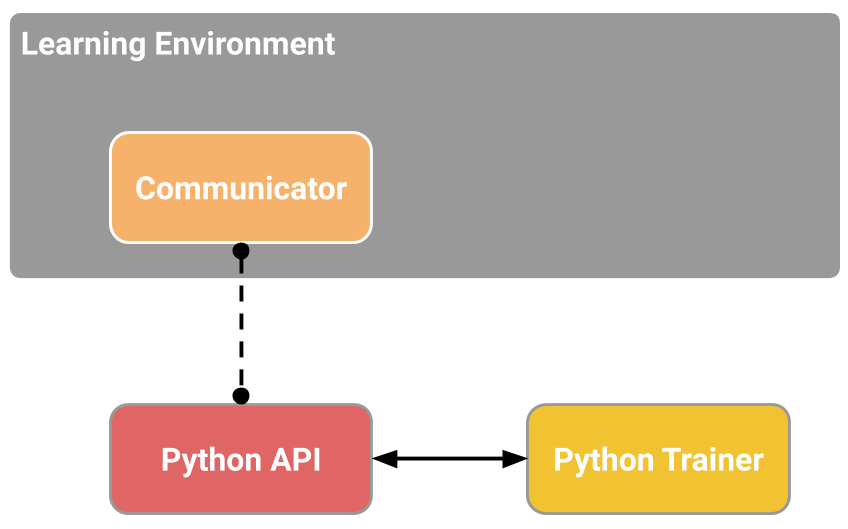
\includegraphics[width=15cm]{resources/figures/learning_environment_basic.png}
\caption{Diagram komponentów Unity ML-Agents}
\label{UnityMlaComponents}
\end{center}
\end{figure}

Poprawnie skonfigurowane Środowisko Uczenia musi zawierać następujące elementy:
\begin{enumerate*}
\item Co najmniej jednego Agenta (z ang. \textit{Agent}). Agent to komponent dołączany do obiektu klasy \texttt{GameObject}, umiejscowionego na scenie Unity. Każdy Agent jest instancją klasy dziedziczącej po klasie \texttt{Agent}. Agent zajmuje się generowaniem Obserwacji, wykonywaniem Akcji oraz przydzielaniem Nagród.
\item Co najmniej jednego Zachowania (z ang. \textit{Behavior}). Zachowanie definiuje określone atrybuty Agenta, takie jak liczba i rodzaj wykonywanych Akcji. Każde Zachowanie jest jednoznacznie identyfikowane poprzez pole \texttt{Behavior Name}. \\
Istnieją trzy rodzaje Zachowań:
\begin{itemize*}
\item Zachowanie Uczące (z ang. \textit{Learning Behavior}) - Zachowanie które musi się wyuczyć. Tego Zachowania używamy podczas treningu sieci neuronowych;
\item Zachowanie Heurystyczne (z ang. \textit{Heuristic Behavior}) - Zachowanie zdefiniowane przez reguły zapisane bezpośrednio w kodzie źródłowym. Przydatne m.in. przy testowaniu nowego Środowiska Uczenia przed rozpoczęciem treningu sieci.
\item Zachowanie Wnioskujące (z ang. \textit{Inference Behavior}) - Zachowanie wykorzystujące wytrenowany model sieci neuronowej. W gruncie rzeczy, Zachowanie Uczące po skończonym treningu sieci neuronowej zmienia się w Zachowanie Wnioskujące.
\end{itemize*}
\end{enumerate*}

\begin{figure}[h]
\begin{center}
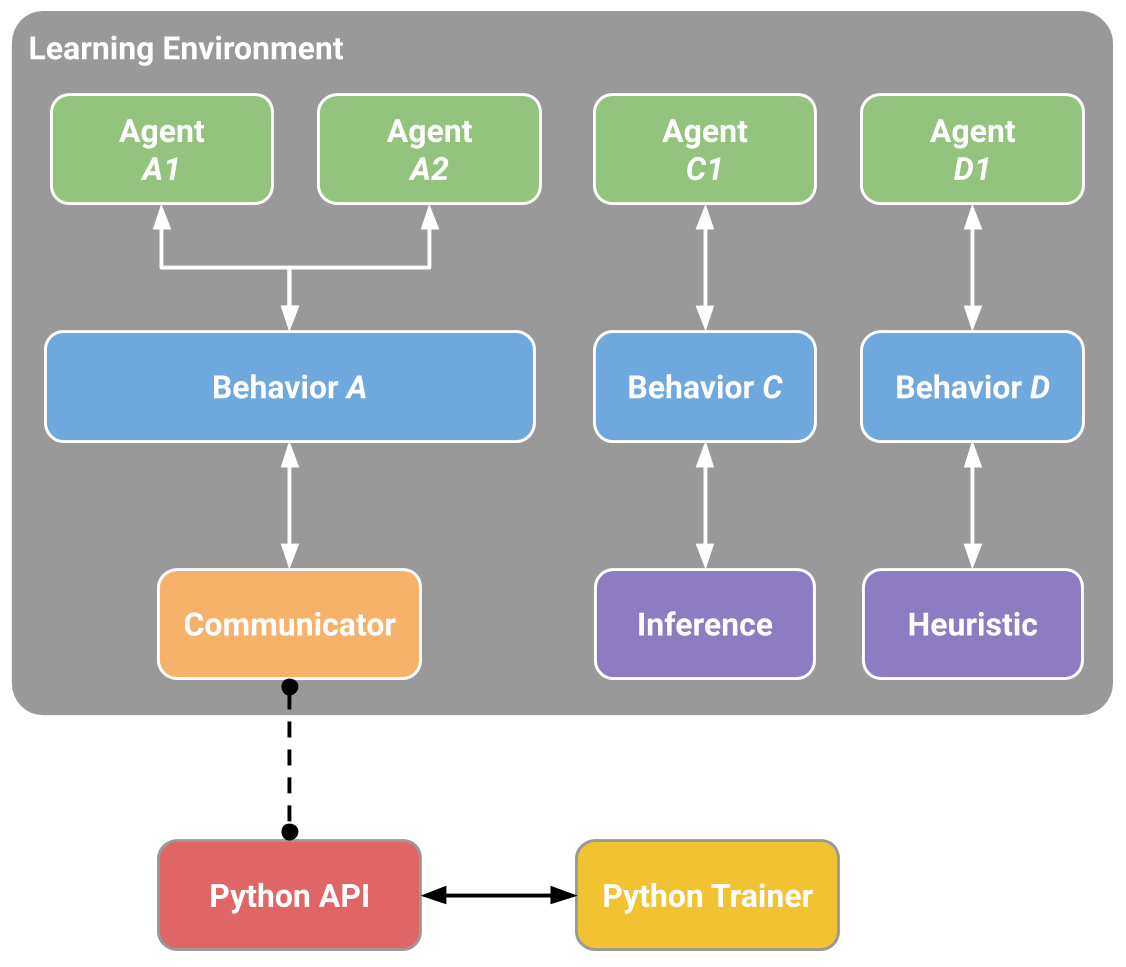
\includegraphics[width=15cm]{resources/figures/learning_environment_example.png}
\caption{Przykład relacji Agentów z Zachowaniami w Środowisku Uczenia}
\label{UnityMlaExample}
\end{center}
\end{figure}

Każdy Agent musi być powiązany z dokładnie jednym Zachowaniem, a Zachowanie może być połączone z więcej niż jednym Agentem. Agenci działający wedle tej samej logiki powinni być powiązani z tym samym Zachowaniem. To wcale nie oznacza, że wszyscy Agenci powiązani z tym samym Zachowaniem muszą współdzielić ze sobą te same Obserwacje, Akcje i Nagrody.

Rysunek \ref{UnityMlaExample} przedstawia przykładowy diagram zależności Agentów z Zachowaniami w Środowisku Uczenia. Agenci \texttt{A1} i \texttt{A2} są podłączeni do Zachowania Uczącego. Agenci \texttt{C1} i \texttt{D1} są podłączeni odpowiednio do Zachowania Wnioskującego i Heurystycznego.

Opisując narzędzie Unity ML-Agents, należałoby również wspomnieć kilka słów o samym Agencie. Każdy Agent wykonuje cyklicznie trzy czynności: generuje Obserwacje, wykonuje zlecone Akcje i oblicza wartość Nagrody. Omówmy każdy z tych elementów:
\begin{enumerate*}
\item Obserwacje (z ang. \textit{Observations}) - zestaw danych wejściowych, niezbędnych do wykonania zleconego Agentowi zadania. Obserwacje mogą być generowane na kilka sposobów:
\begin{itemize*}
\item Nadpisanie metody \texttt{Agent.CollectObservations()} i przesłanie obserwacji do dostarczonego (przez parametr metody) obiektu klasy \texttt{VectorSensor}. Ten sposób najlepiej wykorzystać do aspektów środowiska które można opisać numerycznie i niewizualnie.
\item Dodanie atrybutu \texttt{[Observable]} do pól i właściwości Agenta. Atrybut \\ \texttt{[Observable]} wspiera obecnie podstawowe typy danych (takie jak  \texttt{int}, \texttt{float} czy \texttt{bool}), jak również klasy \texttt{Vector2}, \texttt{Vector3}, \texttt{Vector4}, \texttt{Quaternion} oraz typy enumeracyjne.
\item Implementacja interfejsu \texttt{ISensor}, korzystając z \texttt{SensorComponent} dołączanego do Agenta. Obecnie istnieje kilka implementacji komponentu \texttt{SensorComponent} dostarczanych przez API zestawu Unity ML-Agents. Najważniejsze z nich to:
\begin{itemize*}
\item \texttt{CameraSensorComponent} - używa obrazów z kamery jako obserwacji;
\item \texttt{RenderTextureSensorComponent} - używa zawartości \texttt{RenderTexture} \cite{unity:renderTexture} jako obserwacji;
\item \texttt{RayPerceptionSensorComponent} - używa informacji z zestawu promieni (z ang. \textit{ray casts}) jako obserwacji.
\end{itemize*}
\end{itemize*}
\item Akcje (z ang. \textit{Actions}) - instrukcje zachowań, które Agent powinien wykonać. Istnieją dwa typy Akcji - Ciągłe (z ang. \textit{Continuous}) oraz Nieciągłe (z ang. \textit{Discrete}). Wszystkie Akcje muszą być zdefiniowane w metodzie \texttt{OnActionReceived()}. Akcje Ciągłe to wartości ze zbioru liczb rzeczywistych, podczas gdy Akcje Nieciągłe są wartościami całkowitymi.
\item Nagrody (z ang. \textit{Rewards}) - informacja zwrotna, pozwalająca ocenić jak dobre (lub złe) są Akcje wykonywane obecnie przez Agenta. System Nagród jest najważniejszym elementem w uczeniu ze wzmocnieniem, ponieważ sposób jego skonstruowania ma decydujący wpływ na to, czy trening sieci neuronowej się powiedzie.
\end{enumerate*}

\subsection{Vehicle Physics Pro}
Zaawansowany zestaw do symulacji pojazdów dla silnika Unity 3D. VPP zapewnia wydajny, w pełni realistyczny i dokładny model dynamiki dla niemal każdego typu pojazdu i konfiguracji. W skład zestawu wchodzą m.in. \cite{vpp:features}:
\begin{enumerate*}
\item Wierne odwzorowanie pracy podzespołów pojazdu, obejmujące m.in.:
\begin{itemize*}
\item pracę silnika (spalinowego lub elektrycznego),
\item pracę skrzyni biegów (manualnej lub automatycznej),
\item pracę układu kierowniczego;
\end{itemize*}
\item Symulacja systemów wspomagania jazdy, w tym:
\begin{itemize*}
\item ABS (Anti-lock Braking System),
\item TCS (Traction Control System),
\item ESC (Electronic Stability Control);
\end{itemize*}
\item Liczne rozszerzenia i dodatki, takie jak:
\begin{itemize*}
\item efekty wizualne (np. animacja deski rozdzielczej),
\item efekty dźwiękowe (np. dźwięk silnika),
\item zaawansowana diagnostyka pojazdu, obejmująca m.in. pomiary telemetryczne,
\item system nagrywania, odtwarzania i zapisu powtórek wideo;
\end{itemize*}
\item System zniszczeń wizualnych i mechanicznych;
\item Obsługa szerokiej gamy urządzeń wejściowych, takich jak gamepady czy kierownice do gier wyścigowych;
\item Szczegółowa dokumentacja.
\end{enumerate*}

Większość aspektów symulacji podlega możliwościom dostosowania do potrzeb użytkownika.

\subsection{Conda}
System zarządzania pakietami i środowiskami, posiadający wsparcie dla wielu języków programowania, m.in.: Python, Scala, Java, Fortran \cite{conda:overview}. Conda pozwala łatwo tworzyć, zapisywać i ładować środowiska uruchomieniowe oraz sprawnie przełączać się pomiędzy nimi. Wykorzystując zaledwie kilka prostych poleceń, użytkownik jest w stanie skonfigurować całkowicie odrębne środowisko do uruchomienia wybranej wersji Pythona z określonymi pakietami dodatkowymi. Każde środowisko może posiadać całkowicie odmienną konfigurację.

\subsection{Netron}
Przeglądarka sieci neuronowych \cite{netron:github}. Netron posiada wsparcie dla wielu popularnych technologii wykorzystywanych w uczeniu maszynowym, takich jak ONNX, Keras, czy Barracuda. Ten program jest przeze mnie wykorzystywany do wizualizacji sieci neuronowych, otrzymanych w wyniku przeprowadzenia serii eksperymentów obliczeniowych.

\vspace{0.5cm}

\subsection{Wykorzystane wersje oprogramowania}
\begin{enumerate*}
\item Unity - 2020.3.28f
\item C\# - Mono 6.12.0.122
\item Unity ML-Agents - 0.28.0
\item Vehicle Physics Pro - 9.2
\item Conda - 4.9.2
\item Netron - 5.7.6
\end{enumerate*}

\vspace{0.5cm}

\subsection{Specyfikacja techniczna stacji roboczej}
Oto specyfikacja techniczna stacji roboczej (komputera), na którym została wykonana implementacja systemu oraz zostały przeprowadzone wszystkie eksperymenty obliczeniowe:
\begin{enumerate*}
\item Typ urządzenia - Laptop
\item Marka i model urządzenia - Dell Inspiron 7559 \cite{dellInspiron:specs}
\item Procesor - Intel® Core™ i7-6700HQ (2.6 GHz) \cite{intelCpu:specs}
\item Pamięć RAM - SODIMM DDR3 Synchronous 1600 MHz (32 GB)
\item Karty graficzne:
\begin{itemize*}
\item nVidia GeForce GTX 960M \cite{nvidiaGPU:specs}
\item Intel HD Graphics 530
\end{itemize*}
\item Dysk - PLEXTOR PX-512M7 (SSD 512 GB)
\item System operacyjny - Linux Mint 19.1 Tessa
\end{enumerate*}